\documentclass[11pt, oneside, twocolumn]{article}   	% use "amsart" instead of "article" for AMSLaTeX format
\usepackage[margin=0.75in]{geometry}                		% See geometry.pdf to learn the layout options. There are lots.
\geometry{letterpaper}                   		% ... or a4paper or a5paper or ... 
%\geometry{landscape}                		% Activate for rotated page geometry
%\usepackage[parfill]{parskip}    		% Activate to begin paragraphs with an empty line rather than an indent
\usepackage{graphicx}				% Use pdf, png, jpg, or eps§ with pdflatex; use eps in DVI mode
\graphicspath{ {Figures/} }								% TeX will automatically convert eps --> pdf in pdflatex		
\usepackage{amssymb}
\usepackage[english]{babel}
\usepackage{csquotes}
\usepackage{amsmath}

\usepackage[backend=biber]{biblatex}
\addbibresource{basic.bib}

%SetFonts

%SetFonts


\title{Deep IV GWAS: Milestone \\
	\large Category: Health / Genomics}
\author{
	Jack Andraka\\ 
	\texttt{jandraka@stanford.edu}
	\and
	Billy Ferguson\\
	\texttt{billyf@stanford.edu}
	\and
	Charlie Walker\\
	\texttt{cwalker4@stanford.edu}
}
\date{}							% Activate to display a given date or no date

\begin{document}
\maketitle
\section{Introduction}
Breast cancer accounts for over 25\% of cancer diagnoses and 15\% of cancer-related deaths in women.\textsuperscript{[1]} Ten percent of women with breast cancer have a family history of disease. Women with one premenopausal first-degree relative with breast cancer are at 3.3-fold greater risk than women without a family history,\textsuperscript{[2]} demonstrating that there is a significant genetic contribution to breast cancer risk. To identify genetic factors associated with breast cancer, early studies employed linkage analysis and positional cloning in families with a familial history of breast cancer to discover highly penetrant susceptibility genes such as BRCA1\&2.\textsuperscript{[3]} Although these initial studies were successful and could explain about 20\% of the familial risk of breast cancer,\textsuperscript{[4]} they provided little insight into the role of genetics in nonfamilial breast cancer. \\

More recently, genome-wide association studies (GWAS) have identified over 80 loci significantly associated with sporadic breast cancer. However, these variants collectively only explain 16\% of breast cancer heritability.\textsuperscript{[5]} The inability of GWAS to identify a greater proportion of the genetic risk stems from many factors, including genotyping platform limitations in interrogating rare variation (primarily due to the running of several thousand to several million t-tests simultaneously). This is in contrast with the current hypothesis of genetic architecture that posits many gene variants acting in tandem to produce a phenotypic trait, each with small effect size.\textsuperscript{[6]} The GWAS study design is also plagued by confoundedness, despite the development of many sophisticated statistical techniques to deal with complicated interactions. Simple prediction and correlation setups in breast cancer studies fail to account for this confoundedness (gene expression results in cancerous growth and cancerous growth impacts gene expression). \\

Instrumental variables (IV) have proven to be an adept statistical method for addressing these issues of confoundedness. As shown in Figure 1, IV uses an exogenous instrument $z$ to identify direct causal relationships between some policy variable $p$ on outcome $y$ (a relationship confounded by latent effects $e$). In the case of genetics studies, Mendelian randomization of genetic variants offer up a promising instrument for estimating causal effects of gene expression on cellular phenotype, in this case if the cell is cancerous or not.\textsuperscript{[7]} In this manner, it is possible to identify low-signal, rare variants that would typically not appear in GWAS analyses, thus providing a more comprehensive mapping of the transciptome of a cell to carcinogenesis. \\

Traditional IV experimental designs suffers from the limitation that they require a strong prior understanding of the data generating process (DGP), and are limited in accounting for complex interactions between covariates. Neural networks offer up a solution to this limitation, due to their ability to uncover complicated interactions between genes that are both near and distal.\textsuperscript{[8]} This project provides a proof-of-concept implementation of the Deep-IV framework, applied to characterizing the causal effect of gene expression on carcinogenesis in breast cancer using random, simple nucleotide variants (SNVs). 



\section{Algorithm}
\subsection{Overview}
We implement the method described in ``Deep IV: A Flexible Approach for Counterfactual Prediction'' to identify the effect of a policy variable $p$ on outcome $y$ under confoundedness.\textsuperscript{[9]} Instrumental variables (IV) are a well-developed tool for remedying endogeneity, but require a strong prior understanding of the data generating process and are not well equipped to deal with a large number of covariates. Deep IV promises to marry the best qualities of DNNs and IV, and we believe GWAS are a prime use case. \\

To perform IV analysis one needs to find an exogenous variable that affects the outcome variable only through the endogenous covariate of interest. More specifically, the instrument \emph{z} must be conditionally independent of the error (Figure 1).\\

\begin{figure}[h]
	\caption{Generalized Deep IV}
	\centering
	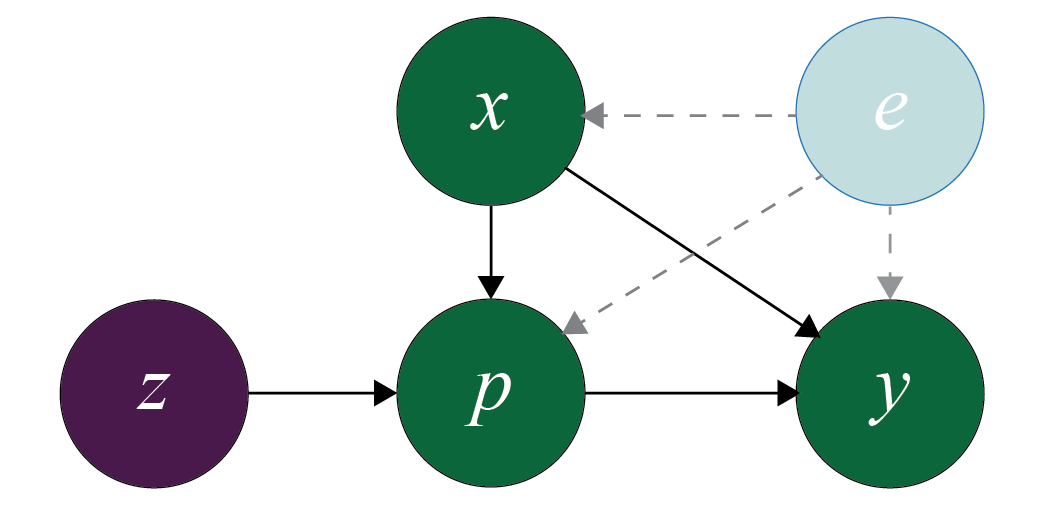
\includegraphics[width=0.5\textwidth]{Figure_1.png}
\end{figure}

Traditional IV can be estimated through a procedure called two-stage least squares (2SLS): in the first stage you regress your endogenous variable of interest, $p$,  on the exogenous instrument, $z$, to create a predicted $\hat{p}$ constructed only with the exogenous variation of $z$. In the second stage, you regress your outcome variable, $y$, on the predicted $\hat{p}$ from the first stage.\footnote{Chapter 4 of Angrist and Pischke's \emph{Mostly Harmless Econometrics: an Empiricist's Companion} provides a good introduction to instrumental variables.}\\

\subsection{Model Architectures}

To adapt this procedure for the DeepIV method, we replace the two-stage least squares with two-stage multilayer perceptrons. We call the first stage our \emph{policy network} and the second our \emph{response network}. Our first iteration is modeled off of the specification in the appendix of the seminal DeepIV paper from Hartford et al. (2017).\textsuperscript{[10]}\\

The policy and response networks in our simulations below have three hidden layers with 128, 64, and 32 hidden units respectively. The policy network takes in the exogenous $z$ and control variables $x$ as input to predict $p$ using tanh acitvation functions for each layer and a Mixture of Gaussian output with 10 components. The predicted $\hat{p}$ from the policy network and $x$ are then fed into the response network to yield predictions $\hat{y}$. The repsone network performs ReLU activation functions for the three hidden layers and linear activation for the output. \\

Both networks use Adam Optimization with learning rate $=0.001$, $\beta_1 = 0.9$, $\beta_2 = 0.999$, and $\epsilon = 1e-08$. For training we use L2 weight decay with penalty parameter $0.001$, a dropout rate of $\textrm{min}(1000/(1000+n); 0.5)$, $(1.5 \times 10^6/n)$ epochs, and batch size $100$. 


\section{Experiment}
\subsection{Motivation and Design}
As a proof-of-concept, we evaluate our approach on simulated data, testing DeepIV's ability to recover an underlying causal relationship in a low-dimensional domain. We compared our DeepIV architecture to a single-stage feed-forward network with the same architecture as our  DeepIV \emph{response} stage. 

\subsection{Simulated Data}
Our simulation models a DGP similar to that described in Section 2. For ease of explanation, we ground our simulation in a typical real-world IV application: estimating the effect of price on sales of some product (say, hotel bookings). We begin by assuming seven customer types, $s \in \{1,...,7\}$ which each exhibit different levels of price sensitivity. Customer price sensitivity varies according to a complex non-linear function of time.
\begin{gather*}
\psi_t = 2\big((t-5)^4/600 + \textrm{exp}\big[-4(t-5)^2\big] + t/10 - 2 \big)\\
t \sim \textrm{unif}(0,10)
\end{gather*}
Prices are a function of observed variable $t$ and some instrument $z$, on the basis that the hotel chooses their price to move with average price sensitivity. In the hotel example, the high demand resulting from some unobserved confounding variable (e.g. a nearby conference) breaks the conditional independence between our policy variable $p$ (price) and the latent effects $e$. We model this by generating our errors $e$ with parameter $\rho$ that denotes the correlation between $p$ and $e$; in other words, it reflects the extent of endogeneity in our population model. Our outcome variable $y$ (sales) is then generated as:
\begin{gather*}
y = 100 + (100 + p)s\psi_t - 2p + e \\
p = 25 + (z + 3)\psi_t + v \\
z, v \sim \mathcal{N}(0,1) \\
e \sim \mathcal{N}(\rho v, 1 - \rho^2)
\end{gather*}
The causal relationship we wish to uncover is $h(t, s, p) = (10 + p)s\psi_t - 2p$, but the correlation between the error $e$ and $p$ in our population model violates the unconfoundedness assumption necessary for causal interpretation. \\

Since we have our ground truth causal relationship, we evaluate our model by first generating features $[t, s, p]$, but then change $p$ to a fixed grid of price values $p'$. This allows us to compare our predicted sales, $\hat{h}$ against the ground truth $h$. 

\subsection{Results} 
Results of @billyf and @cwalker4 simulations.

\section{Data}
@jandraka

\section{Next Steps}
This milestone was a proof of concept, showing that the DeepIV method effectively uncovers causal relationships that are glossed over by a naive Feed Forward Neural Net. Crucially, first implementing our architecture on simulated data provided a sanity check of our code before moving forward with our real life dataset where the true causal relationship is unknown.

Just recently we were granted access to breast cancer genetic data. The path forward entails cleaning this data, running our baseline model described above on the genetic data, and then tuning our hyperparameters. Additionally, we would like to include the standard 2SLS as another baseline to judge the effectiveness of the DeepIV architecture against the standard IV method. 

\pagebreak
\onecolumn
\begin{thebibliography}{9}
\bibitem{1} 
Torre, L. A., et al.
\textit{Global Cancer Incidence and Mortality Rates and Trends--An Update.}
Cancer Epidemiology Biomarkers and Prevention, vol. 25, no. 1, 2015, pp. 16–27.
\bibitem{2} 
Spicer, D.
\textit{Risk Factors for Development of Breast Cancer}.
Breast Cancer, 2005, pp. 49–57.
\bibitem{3} 
Joosse, Simon A.
\textit{BRCA1 And BRCA2: a Common Pathway of Genome Protection but Different Breast Cancer Subtypes}.
Nature Reviews Cancer, vol. 12, no. 5, 2012, pp. 372–372.
\bibitem{4} 
Thompson, Deborah, and Douglas Easton.
\textit{The Genetic Epidemiology of Breast Cancer Genes}.
Journal of Mammary Gland Biology and Neoplasia, vol. 9, no. 3, 2004, pp. 221–236.
\bibitem{5} 
Skol, Andrew D., et al.
\textit{The Genetics of Breast Cancer Risk in the Post-Genome Era: Thoughts on Study Design to Move Past BRCA and towards Clinical Relevance}.
Breast Cancer Research, vol. 18, no. 1
\bibitem{6} 
Campos, Gustavo De Los, et al.
\textit{Predicting Genetic Predisposition in Humans: the Promise of Whole-Genome Markers}.
Nature Reviews Genetics, vol. 11, no. 12, 2010, pp. 880–886.
\bibitem{7} 
Burgess, Stephen, et al.
\textit{Dissecting Causal Pathways Using Mendelian Randomization with Summarized Genetic Data: Application to Age at Menarche and Risk of Breast Cancer}.
Genetics, vol. 207, no. 2.
\bibitem{8} 
Cheng, Long, et al.
\textit{Recurrent Neural Network for Non-Smooth Convex Optimization Problems With Application to the Identification of Genetic Regulatory Networks}.
IEEE Transactions on Neural Networks, vol. 22, no. 5, 2011, pp. 714–726.
\bibitem{9} 
Harford, Jason, et al.
\textit{Deep IV: A Flexible Approach for Counterfactual Prediction}.
International Conference on Machine Learning. 2017. 
\bibitem{10} 
Harford, Jason, et al.
\textit{Appendix for Deep IV: A Flexible Approach for Counterfactual Prediction}.
International Conference on Machine Learning. 2017. 

\end{thebibliography}



\end{document}  